\section{Extraction of the structure functions}
\label{sec:structure}
The $\pi^0$ differential cross section in the 
resonance center of mass assumes the form

\begin{equation}
\Dfrac{d\sigma}{d\Omega^*_{\pi^0}} = \Dfrac{2W p^*_{\pi^0}}{W^2-m_P^2}\left( \sigma_T + \epsilon\sigma_L
+\epsilon\sigma_{TT}sin^2\theta cos2\phi +
\sigma_{LT}\sqrt{2\epsilon_L(\epsilon+1)}sin\theta cos\phi \right)
\end{equation}

where  $\phi$ and $\theta$ are the azimuthal and polar angle of the $\pi^0$ in the c.m. frame
and  $\sigma_T$, $\sigma_L$, $\sigma_{LT}$, $\sigma_{TT}$   are the structure functions.
The $\phi$ distributions are modulated only by the terms $\cos\phi$ and $\cos 2\phi$ while all the other
terms vary with $W$, $Q^2$ and $\cos\theta$ (but not with $\phi$).
Therefore the structure functions can be extracted with a $\phi$ fit.

For each $W$, $Q^2$ and $\cos\theta$ bin the 
quantity in parenthesis is fitted with the functional form
\begin{equation}
 y = a + b\cos\phi + c\cos 2\phi
\end{equation}
The structure functions are then calculated with the formulas:
\begin{equation}
\begin{array}{l l l}
\sigma_T + \epsilon\sigma_L & = & a \\
& & \\
\sigma_{LT}                 & = & \Dfrac{b}{\sin\theta\sqrt{2\epsilon_L(\epsilon + 1)}} \\
& & \\
\sigma_{TT}                 & = & \Dfrac{c}{\sin^2\theta \epsilon_T}
\end{array}
\end{equation}
See    \begin{verbatim} 
http://www.jlab.org/~ungaro/pi0eprod/cro_plots
\end{verbatim}
for the cross section plots in each bin considered and for different cuts applied
during this analysis.




\F{fig:bac_phi_W1.23_Q22.40} shows the $\phi$ fits of the cross section for $W=1.1\,\pm\,0.01$ GeV and $Q^2 = 2.4$ GeV$^2$.

\F{fig:chi2_ctr} shows the  $\chi^2/\nu$ distribution for all the fits at different $Q^2$ 
values (black points) along with the expected $\chi^2/\nu$ distribution (red line)
\begin{equation}
\chi^2/\nu(x) = \Dfrac{2}{2^{\nu /2} \Gamma(\nu /2)} \, x^{\nu-1}\, e^{-x^2/2}
\end{equation}



There are 12 bins in $\phi$ and there  are 3 fit paramters therefore
$$
 \nu = {N-{\rm constraints}} = 9.
$$
\F{fig:Sigma_lpt_Q2_2.40} shows $\sigma_L + \epsilon\sigma_T$ resulting from the fit at $Q^2 = 2.4$ GeV$^2$.

\begin{figure}[h]
 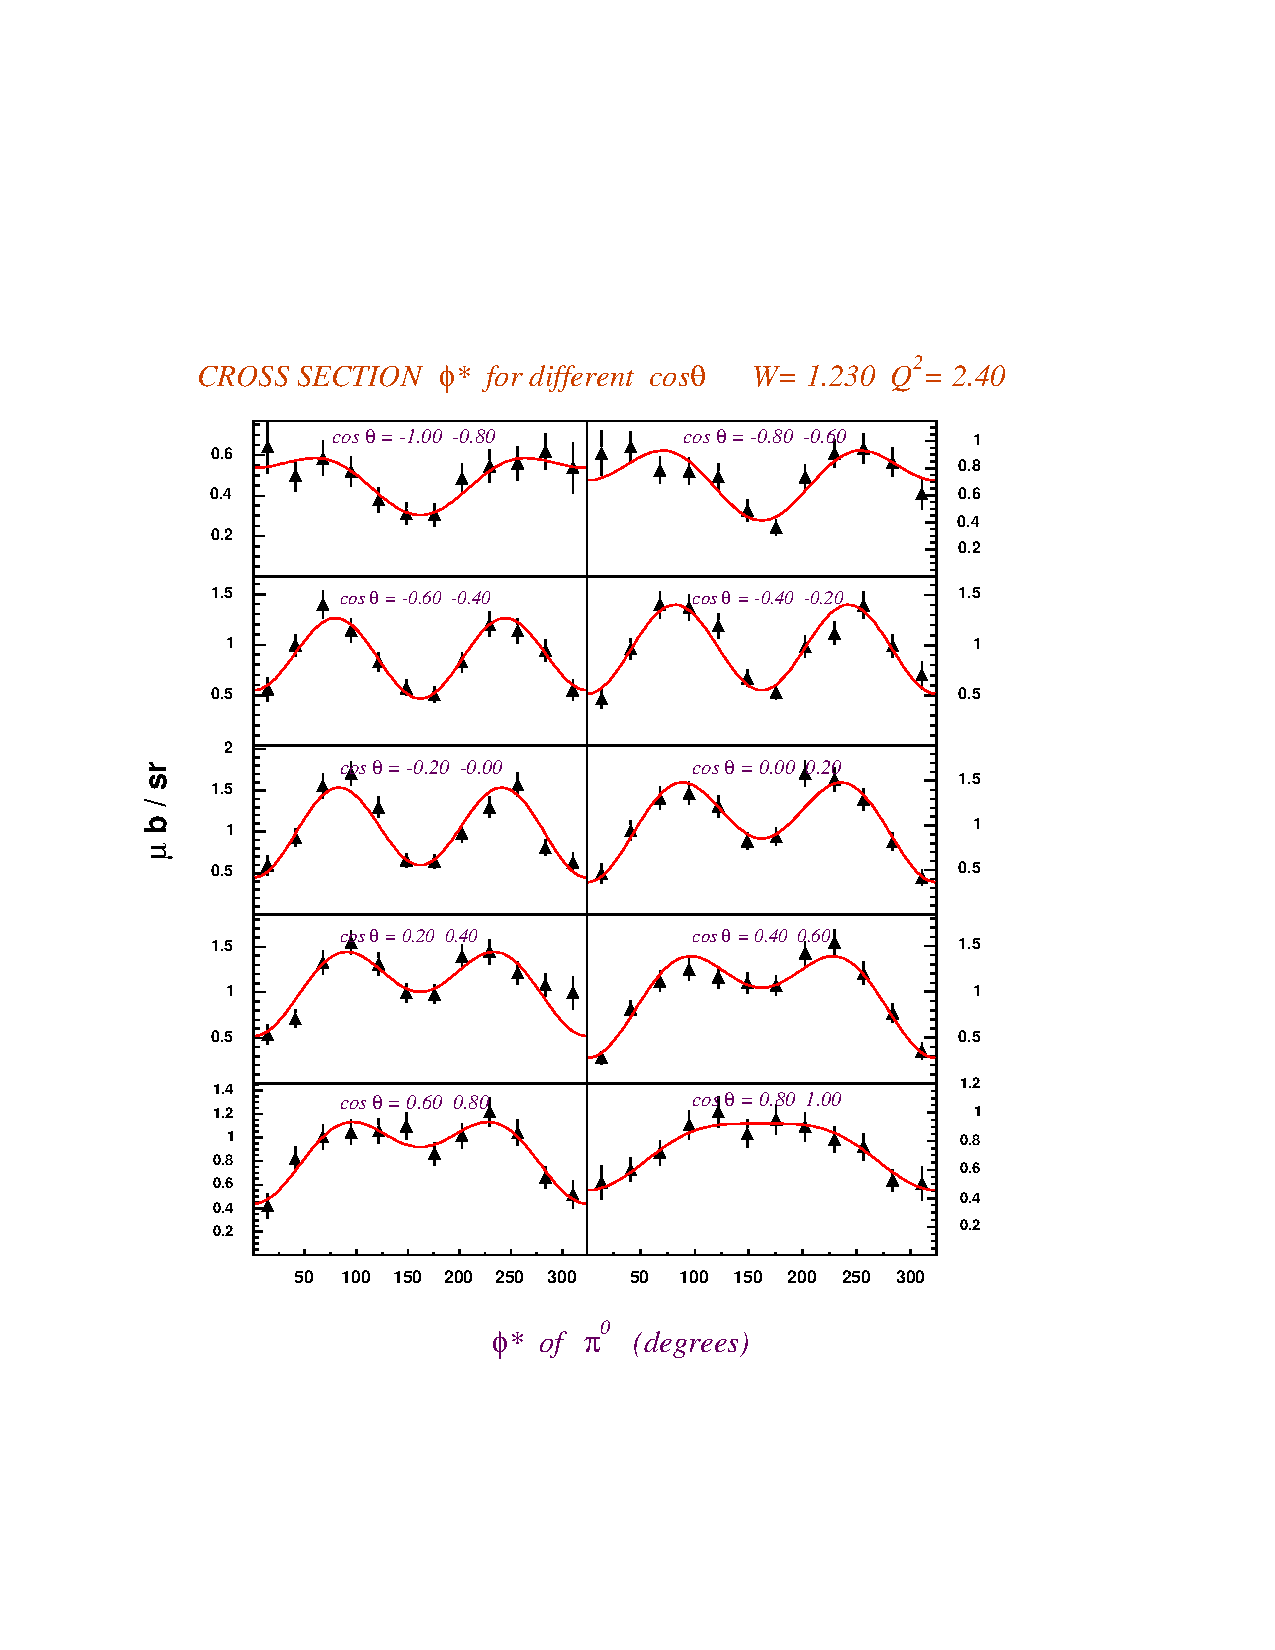
\includegraphics[width = 11cm, bb=60 120 420 640]{analysis/img/bac_phi_W1.23_Q22.40}
  \caption[$\phi$ fits of the cross section for different $\cos\theta$ values]
          { $\phi$ fits of the cross section for different $\cos\theta$ values.
	             The function used for the fit is $ y = a + b\cos\phi + c\cos 2\phi$
		     and the structure functions follow from the parameters $a,b,c$.}
 \label{fig:bac_phi_W1.23_Q22.40}

\end{figure}
\cia

\begin{figure}[h]
 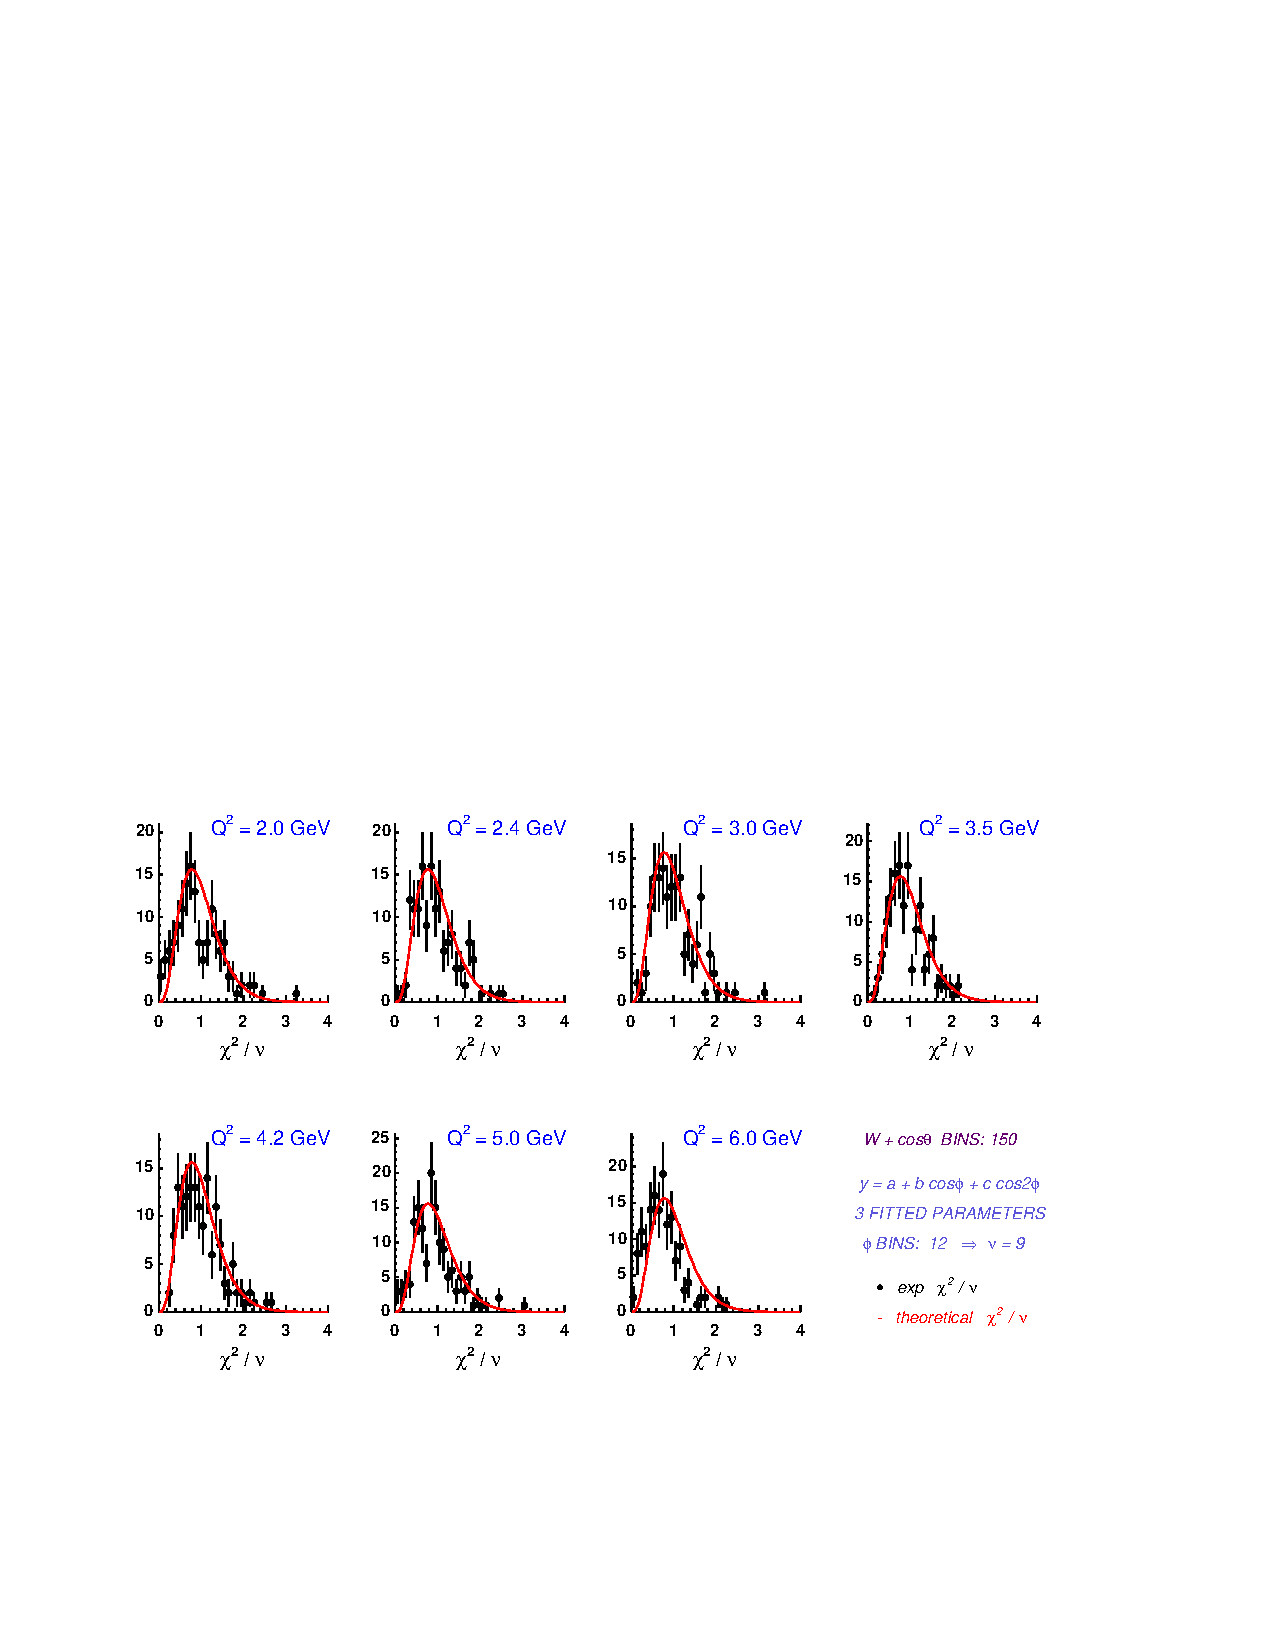
\includegraphics[width = 11cm, bb=50 110 380 400]{analysis/img/chi2_ctr} 
  \caption[Reduced $\chi^2$ distribution of the $\phi$ fits]
          { Reduced $\chi^2$ distribution of the $\phi$ fits. The distributions
	             show consistency with the expected  $\chi^2$ distribution for 150 fits
		     (15 W bins and 10 $\cos\theta$ bins) and 9 degrees of freedom.}
 \label{fig:chi2_ctr}
\end{figure}




